%Diseño de Hardware
\section{Diseño de hardware} % (fold)
\label{sec:diseno_de_hardware}




Con el microcontrolador seleccionado, se procedió a la etapa de diseño de hardware. La placa de desarrollo C8051F350 (Sección \ref{sec:silicon_labs_c8051f352}) con la que se contó en el laboratorio donde se trabajo, sirvió de modelo para delinear el circuito esquemático en la placa a desarrollar.


\subsection{Diagrama de Bloques de Hardware} % (fold)
\label{sub:diagrama_de_bloques_de_hardware}

La primera etapa de diseño consiste en realizar un diagrama de bloques que ilustre a grandes rasgos la organización del circuito. Luego de esto se realiza el diseño esquemático que consiste en llevar cada bloque a nivel de componente electrónico y realizar la interconexión necesaria entre todos los elementos existentes para lograr el funcionamiento buscado. Los diagramas de bloque y esquemáticos se pueden ver en las figuras \ref{fig:bloquesHW} y \ref{fig:esquematico}. Con ayuda del software KiCad$^{\tiny{\cite{bib:kicad}}}$, se realizo el diagrama esquemático y la implementación en circuito impreso correspondiente al esquemático construido.

\begin{figure}[h]
  \centering
  \includegraphics[width=0.80\textwidth, height = 9cm]{bloquesHW}
  \caption{\small Diagrama de bloques del circuito a realizar}\label{fig:bloquesHW}
\end{figure}

Los bloques en la figura \ref{fig:bloquesHW} representan de forma general los distintos módulos a implementar. Las entradas analógicas se introducen al sistema a través de filtros reductores del ruido. Luego, las señales, ingresan al microcontrolador para ser procesadas por él mismo. El bloque de GPIO y contadores de eventos es simplemente un grupo de pines direccionados a distintas entradas del microcontrolador. GPIO significa ``General Purpose Input Output''( en español, ``entrada y salida de propósito general'' ). Son 4 pines que se separaron para uso general, por necesidad eventual de necesitarlos. Parte de estos GPIO son los pines contadores de eventos, por lo cual se incluyeron dentro del mismo bloque.

Es posible alimentar el sistema por medio del programador (propietario de Silicon Labs), o mediante una fuente de tension$^{\tiny{\cite{bib:lm2937}}}$ de 3,3V que se obtiene como salida de un regulador de tensión, cuya entrada es de 5V. La llave selectora decide si se alimenta el sistema usando la fuente continua de 5V, o utilizando el programador.

% subsection diagrama_de_bloques_de_hardware (end)



\subsection{Diagrama Esquemático} % (fold)
\label{sub:diagrama_esquematico}

La figura \ref{fig:esquematico} muestra el diagrama esquemático del circuito a implementar. El microcontrolador (Sección \ref{sec:silicon_labs_c8051f352}) con el que se trabaja tiene ciertos niveles de tensión de operación con el que se trabaja. En principio, se alimenta con una fuente de 5V y 500mA que trabaja junto con un regulador de tensión$^{\tiny{\cite{bib:lm2937}}}$ llevando la alimentación a un nivel de 3,3V. Estos 3,3V se utilizan para alimentar al microcontrolador; la tensión analógica positiva del conversor; a un integrado MAX232$^{\tiny{\cite{bib:max232}}}$ que se utiliza para lograr una interfaz serial entre la UART (Sección \ref{sub:interfaz_serial}) de la placa y un puerto serial de una PC; y a un led testigo de alimentación.

\begin{figure}[H]
  \centering
  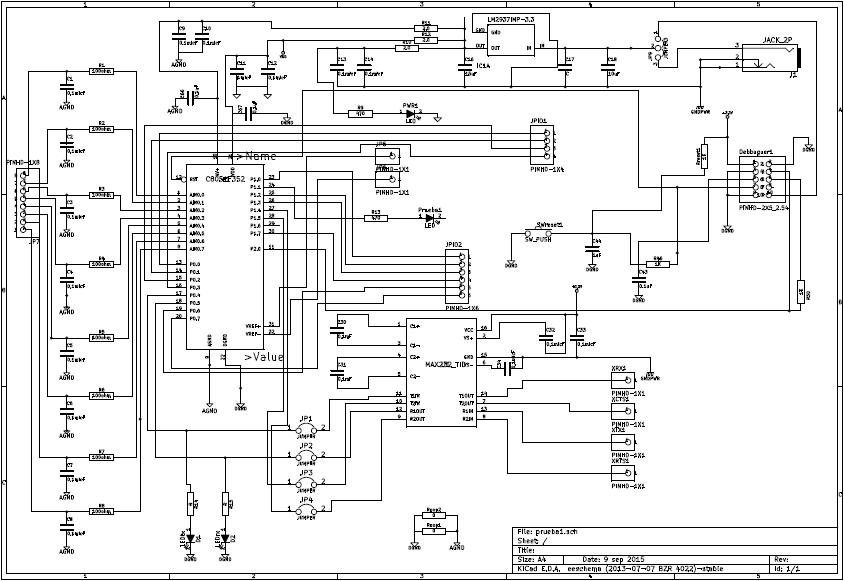
\includegraphics[width=0.95\textwidth, height = 10cm]{esquematico}
  \caption{\small Diagrama esquemático del circuito realizado}\label{fig:esquematico}
\end{figure}

Como podemos ver, el esquemático, es una proyección (a nivel electrónico) del diagrama de bloques. %La idea de este diagrama es que cualquier persona (que tenga conocimientos básicos sobre electrónica) pueda entender las interconexiones, los componentes utilizados y el funcionamiento del hardware. 

% subsection diagrama_esquemático (end)

\subsection{Implementación en Circuito Impreso} % (fold)
\label{sub:implementacion_en_circuito_impreso}

Una implementación en circuito impreso consiste simplemente en pasar de un diagrama esquemático al despliegue físico de los componentes reales en una PCB (en inglés, Printed Circuit Board). Para esto, se utilizaron funcionalidades del software KiCad$^{\tiny{\cite{bib:kicad}}}$, que también se utilizo para realizar el esquemático del circuito. Una imagen del resultado del despliegue de componentes esta en la figura \ref{fig:PCB1}, así con el PCB se utiliza para organizar los componentes y las interconexiones físicas, de modo tal que así quede en la placa impresa.

\begin{figure}[H]
  \centering
  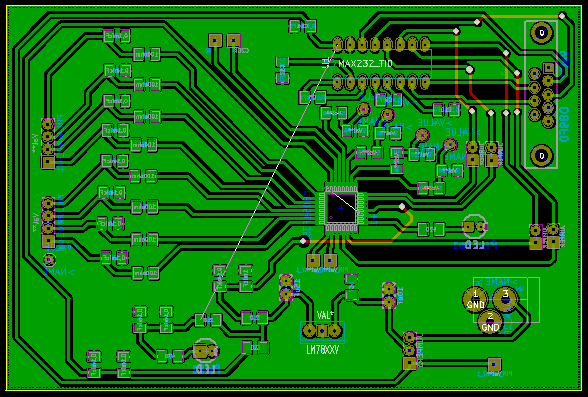
\includegraphics[width=0.95\textwidth, height = 10cm]{PCB1}
  \caption{\small Diagrama del despliegue de componentes}\label{fig:PCB1}
\end{figure}

% subsection implementación_en_circuito_impreso (end)

\subsection{Circuito anexo de programación} % (fold)
\label{sub:circuito_anexo_de_programacion}

Para programar el microcontrolador, se utiliza un programador de la marca de Silicon Labs hecho para la placa de desarrollo utilizada. Es posible usar este mismo programador en la plataforma a construir, pero es necesario armar un circuito que funcione como interfaz entre la placa del microcontrolador y el programador de la misma. El procedimiento para realizar esta placa es el mismo que se utilizó para la del microcontrolador. En la figura \ref{fig:PCB2} se puede ver la figura del despliegue de componentes electrónicos de este circuito.

\begin{figure}[H]
  \centering
  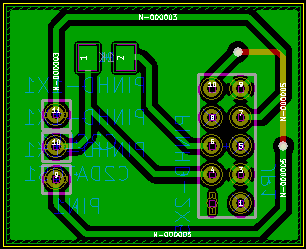
\includegraphics[width=0.20\textwidth, height = 3cm]{PCB2}
  \caption{\small Diagrama del despliegue de componentes del circuito que hace de interfaz entre el programador y la plataforma}\label{fig:PCB2}
\end{figure}

% subsection circuito_anexo_de_programación (end)

\subsection{Impresion del circuito en placa de cobre} % (fold)
\label{sub:impresion_del_circuito_en_placa_de_cobre}

La impresión de la placa física se implemento mas de una vez. El objetivo principal del prototipo era poder correr un programa en el microcontrolador y verificar su funcionamiento. Hubo cuatro prototipos en total. En cada una de ellas salieron a la vista distintos errores que hacían necesaria una nueva impresión para corregirlos.

\subsubsection{Primer prototipo} % (fold)
\label{ssub:primer_prototipo}

La primera versión de la placa se puede ver en la figura \ref{fig:placa1}. En esta primera placa hubo errores de diseño del despliegue de componentes, ya que varias de las pistas se solapaban, y esto hubiese provocado cortocircuito entre las pistas.
\begin{figure}[H]
  \centering
  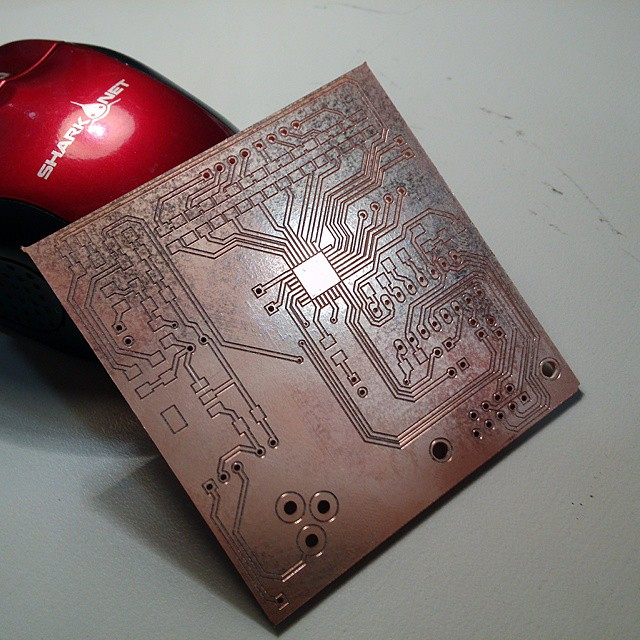
\includegraphics[width=0.60\textwidth, height = 6cm]{placa1}
  \caption{\small Fotografía del primer prototipo}\label{fig:placa1}
\end{figure}


% subsubsection primer_prototipo (end)
\subsubsection{Segundo prototipo} % (fold)
\label{ssub:segundo_prototipo}

En la segunda versión se experimentaron problemas relacionados al ancho de los huecos de las patas de algunos componentes. En particular, el encapsulado del regulador de tensión$^{\tiny{\cite{bib:lm2937}}}$ de 3,3V, encargado de suministrar tensión al microcontrolador, no podía colocarse correctamente en la placa. Al ser una pieza tan importante, dado que sin el el microcontrolador no enciende, hubo que rehacer la placa. Una fotografía del segundo prototipo puede verse en la figura \ref{fig:placa2}.

\begin{figure}[H]
  \centering
  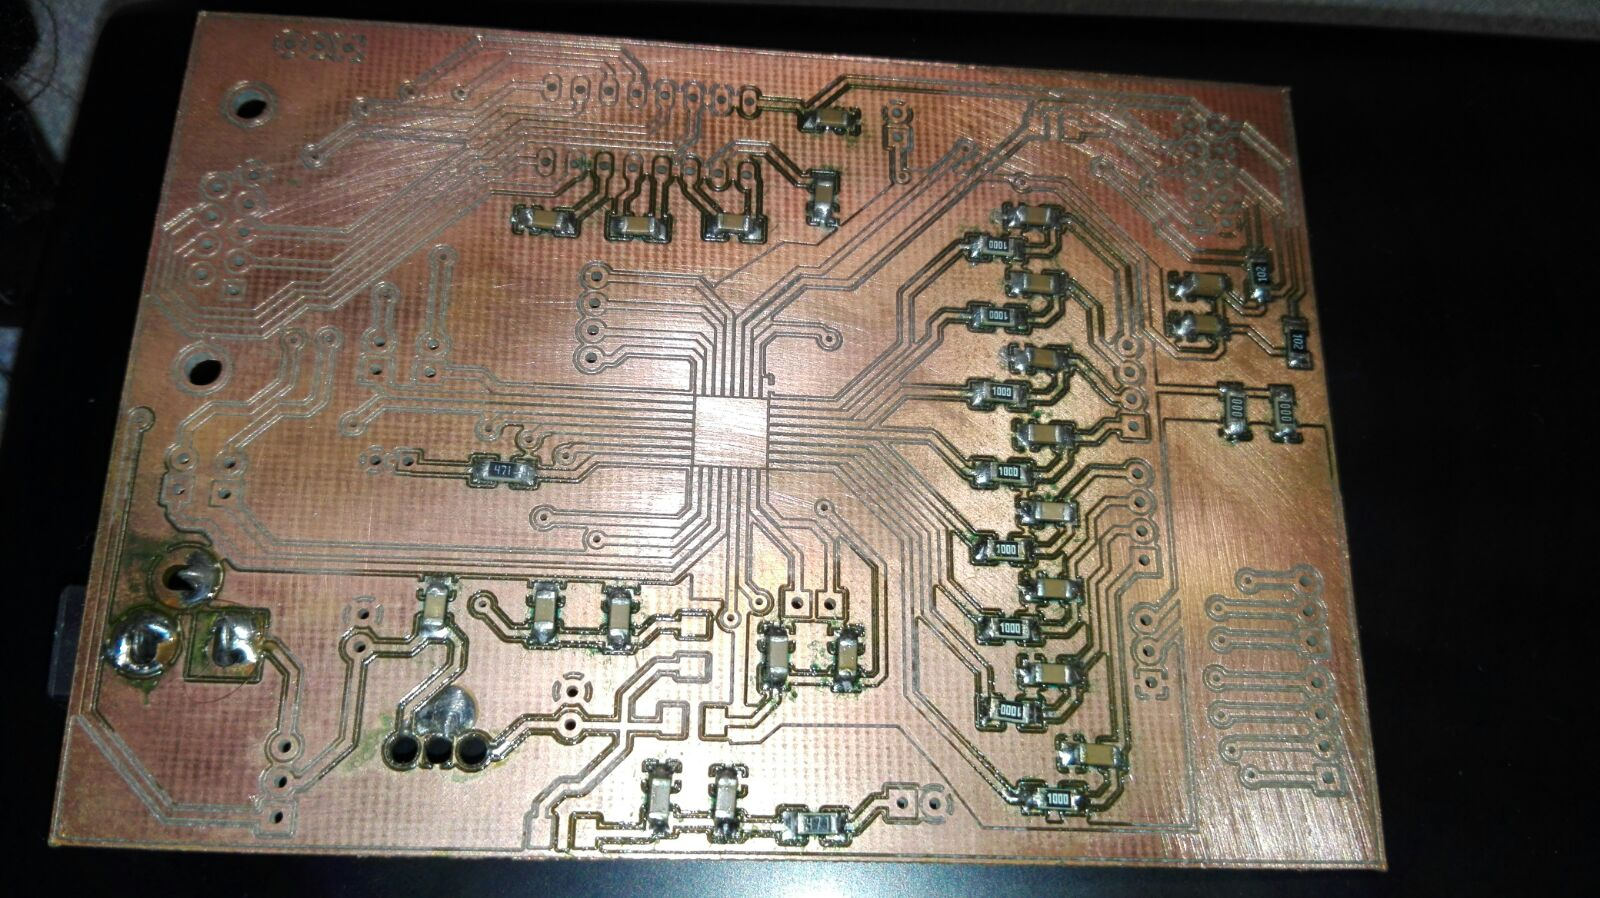
\includegraphics[width=0.60\textwidth, height = 6cm]{placa2}
  \caption{\small Fotografía del segundo prototipo}\label{fig:placa2}
\end{figure}

% subsubsection segundo_prototipo (end)

\subsubsection{Tercer prototipo} % (fold)
\label{ssub:tercer_prototipo}

La figura \ref{fig:placa3} muestra una fotografía del tercer prototipo de la placa. En esta versión el problema se radico en la ficha que se utiliza para la alimentación. Hubo un cortocircuito producto de una mala soldadura, y el microcontrolador se quemo. Cuando se intento remover el chip, las pistas que conectaban al microcontrolador con el resto de los componentes se despegaron de la placa, haciendo que no nos quedé otra alternativa más que realizar una nueva implementación. 
\begin{figure}[H]
  \centering
  \includegraphics[width=0.40\textwidth, height = 5cm]{placa3}
  \caption{\small Fotografía del tercer prototipo}\label{fig:placa3}
\end{figure}


% subsubsection tercer_prototipo (end)

\subsubsection{Cuarto prototipo} % (fold)
\label{ssub:cuarto_prototipo}

Al terminar con la ultima impresión, se encontró con el problema de que el microcontrolador solo lograba conectarse a al programador ocasionalmente, sin seguir un patrón claro. Luego de bastante tiempo buscando el problema se descubrió que, las resistencias que se colocan a la salida del regulador de tensión eran mucho mas grandes que las que se necesitaban (se habían colocado resistencias de 470 Ohm y eran necesario colocar de 2 Ohm). Luego de detectar esto, se desoldaron las resistencias puestas y se colocaron las correctas. Luego la placa conecto correctamente al programador y a la PC. Con esto, se pudo descargar el código realizado al mirocontrolador y ponerlo en funcionamiento. Una fotografía de la ultima implementación puede verse en la figura \ref{fig:placa4}.
\begin{figure}[H]
  \centering
  \includegraphics[width=0.40\textwidth, height = 5cm]{placa4}
  \caption{\small Fotografía del cuarto y último prototipo realizado}\label{fig:placa4}
\end{figure}


% subsubsection cuarto_prototipo (end)